\section{Benchmark NIST-5 "Battery"}
\label{sec:bench-5}

This is a heat conduction problem in a nonhomogeneous material.
It comes with an anisotropic solution with strong internal boundary
layers and multiple singularities.
The solution has multiple point singularities in the interior at which
more than three different materials meet which are stronger than those
corresponding to reentrant corners \cite{demkowicz-1}.
The equation solved is given by

\begin{equation} \label{heat-conduction}
-\frac{\partial }{\partial x}\left(p(x, y)\frac{\partial u}{\partial x}\right)
-\frac{\partial }{\partial y}\left(q(x, y)\frac{\partial u}{\partial y}\right) = f,
\end{equation}

in the domain $\Omega = (0, 8.4) \times (0, 24)$, equipped with
zero Neumann boundary condition on the left edge, Natural boundary
conditions on the rest of the boundary:
\begin{equation}
\left\{
\begin{array}{l}
\displaystyle p(x, y)\frac{\partial u}{\partial x}\nu_1 + q(x, y)\frac{\partial u}{\partial y}\nu_2 = g_{left}(x, y) \ \mbox{on} \  \Gamma_{left} \\
\displaystyle p(x, y)\frac{\partial u}{\partial x}\nu_1 + q(x, y)\frac{\partial u}{\partial y}\nu_2 + c(x, y)u = g_{right}(x, y) \ \mbox{on} \ \Gamma_{right} \\
\displaystyle p(x, y)\frac{\partial u}{\partial x}\nu_1 + q(x, y)\frac{\partial u}{\partial y}\nu_2 + c(x, y)u = g_{top}(x, y) \ \mbox{on} \ \Gamma_{top} \\
\displaystyle p(x, y)\frac{\partial u}{\partial x}\nu_1 + q(x, y)\frac{\partial u}{\partial y}\nu_2 + c(x, y)u = g_{bottom}(x, y) \ \mbox{on} \ \Gamma_{bottom}
\end{array}
\right.
\end{equation}

where $p(x, y)$, $q(x, y)$, $c(x, y)$, $g(x, y)$, and the right hand side $f$ are constant functions (different in respective materials).

The solution of NIST-5 is shown in Fig. \ref{fig:sln-nist05}.

\begin{figure}[!ht]
\centering
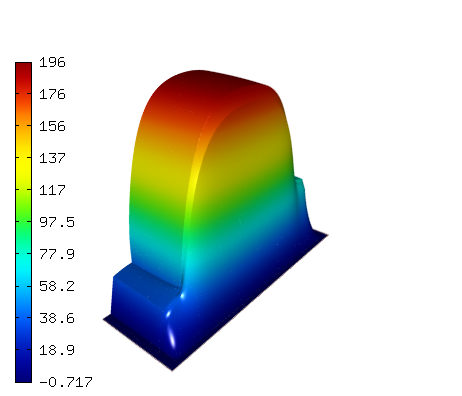
\includegraphics[height=5cm]{nist/nist-5/solution.png}
\caption{The solution to NIST-5 benchmark problem.}
\label{fig:sln-nist05}
\end{figure}

The goal of the benchmark is to reach a relative error below
$0.1$~\% in the $H^1$-norm with as few DOFs as possible.
We begin with adaptive $hp$-FEM,
the initial mesh is shown in Fig. \ref{fig:nist-5-hp-aniso} (left).
In 28 adaptivity steps, the resulting mesh with 2711 DOF is shown
in Fig. \ref{fig:nist-5-hp-aniso} (right).

\begin{figure}[!ht]
\centering
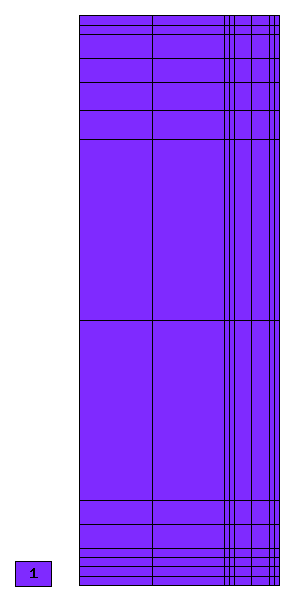
\includegraphics[height=5cm]{nist/nist-5/mesh_hp_aniso_init.png}\ \
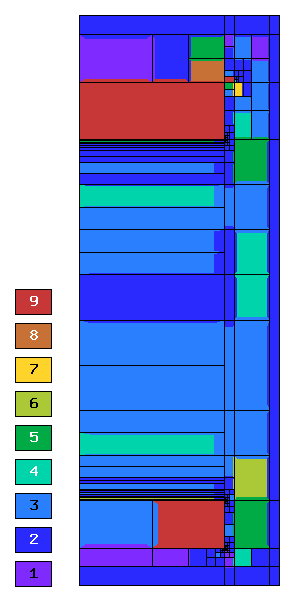
\includegraphics[height=5cm]{nist/nist-5/mesh_hp_aniso.png}
\vspace{-2mm}
\caption{Initial mesh (left) and final mesh (right) for $hp$-FEM with anisotropic refinements.}
\label{fig:nist-5-hp-aniso}
\end{figure}

The final relative error estimate in $H^1$-norm was 9.17542e-02 \%,
and it was identical to the exact error in all printed digits.
We also solved this benchmark with adaptive $h$-FEM
with linear (left) and quadratic (right)
elements, with anisotropic refinements enabled.
Final meshes for the $h$-FEM computations are shown
in Fig. \ref{fig:nist-5-h-aniso}.

\begin{figure}[!ht]
\centering
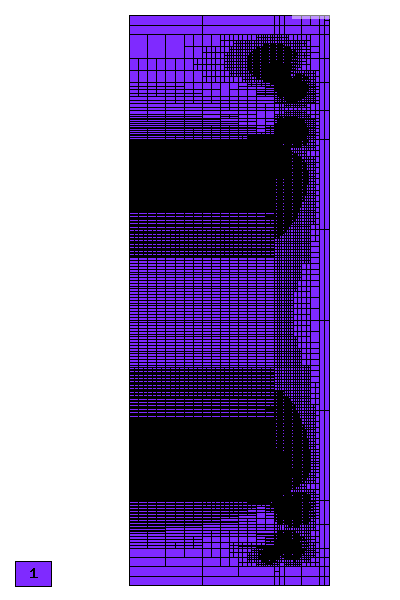
\includegraphics[height=5cm]{nist/nist-5/mesh_h1_aniso.png}\ \
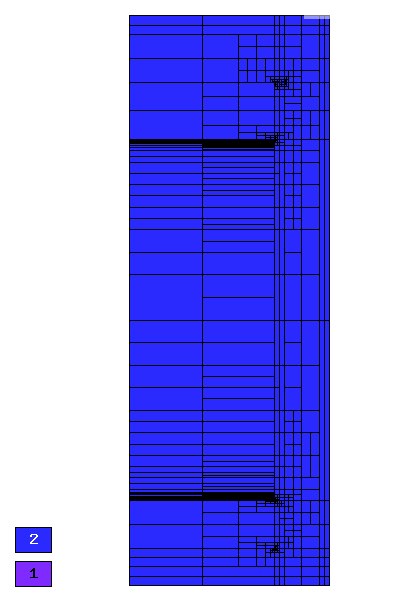
\includegraphics[height=5cm]{nist/nist-5/mesh_h2_aniso.png}
\vspace{-2mm}
\caption{Final mesh for $h$-FEM anisotropic refinements with linear and quadratic elements.}
\label{fig:nist-5-h-aniso}
\end{figure}

Finally, Figs. \ref{fig:nist-5-conv} compare all
three approaches to automatic adaptivity from the point
of view of DOF and CPU convergence.

\begin{figure}[!ht]
\centering
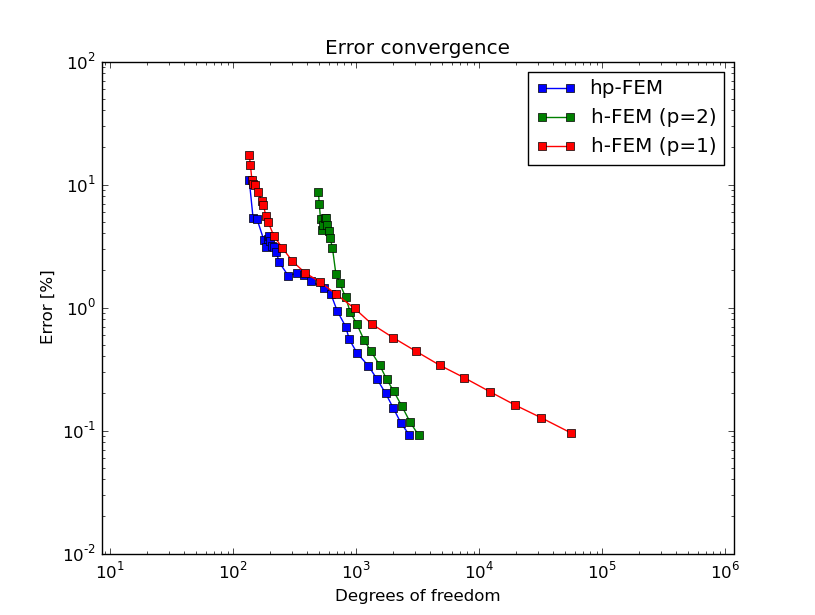
\includegraphics[height=5cm]{nist/nist-5/conv_dof_aniso.png}\ \
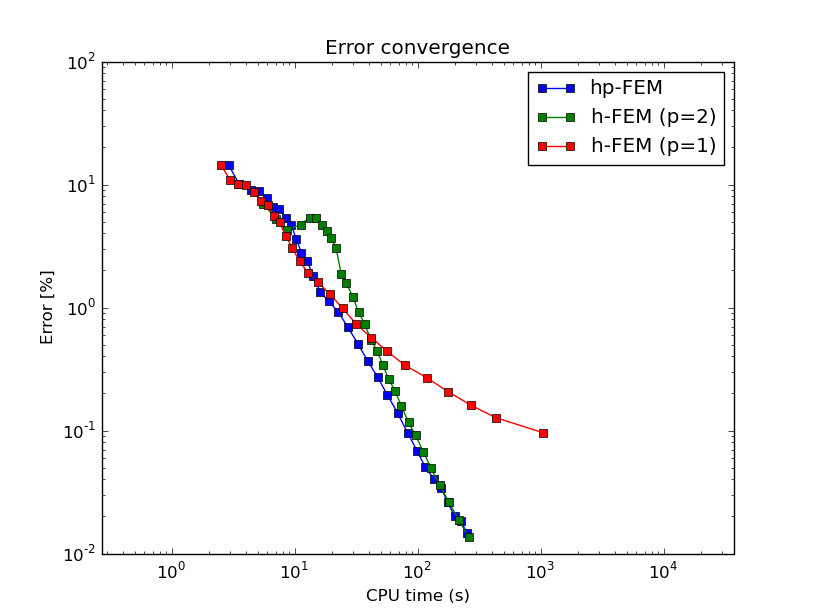
\includegraphics[height=5cm]{nist/nist-5/conv_cpu_aniso.png}
\caption{DOF and CPU time convergence graphs.}
\label{fig:nist-5-conv}
\end{figure}

